\documentclass[tikz,border=1cm]{standalone}
\usepackage{tikz-3dplot,calc}
\usetikzlibrary{shadings}
\pagecolor{green!10}
\begin{document}
	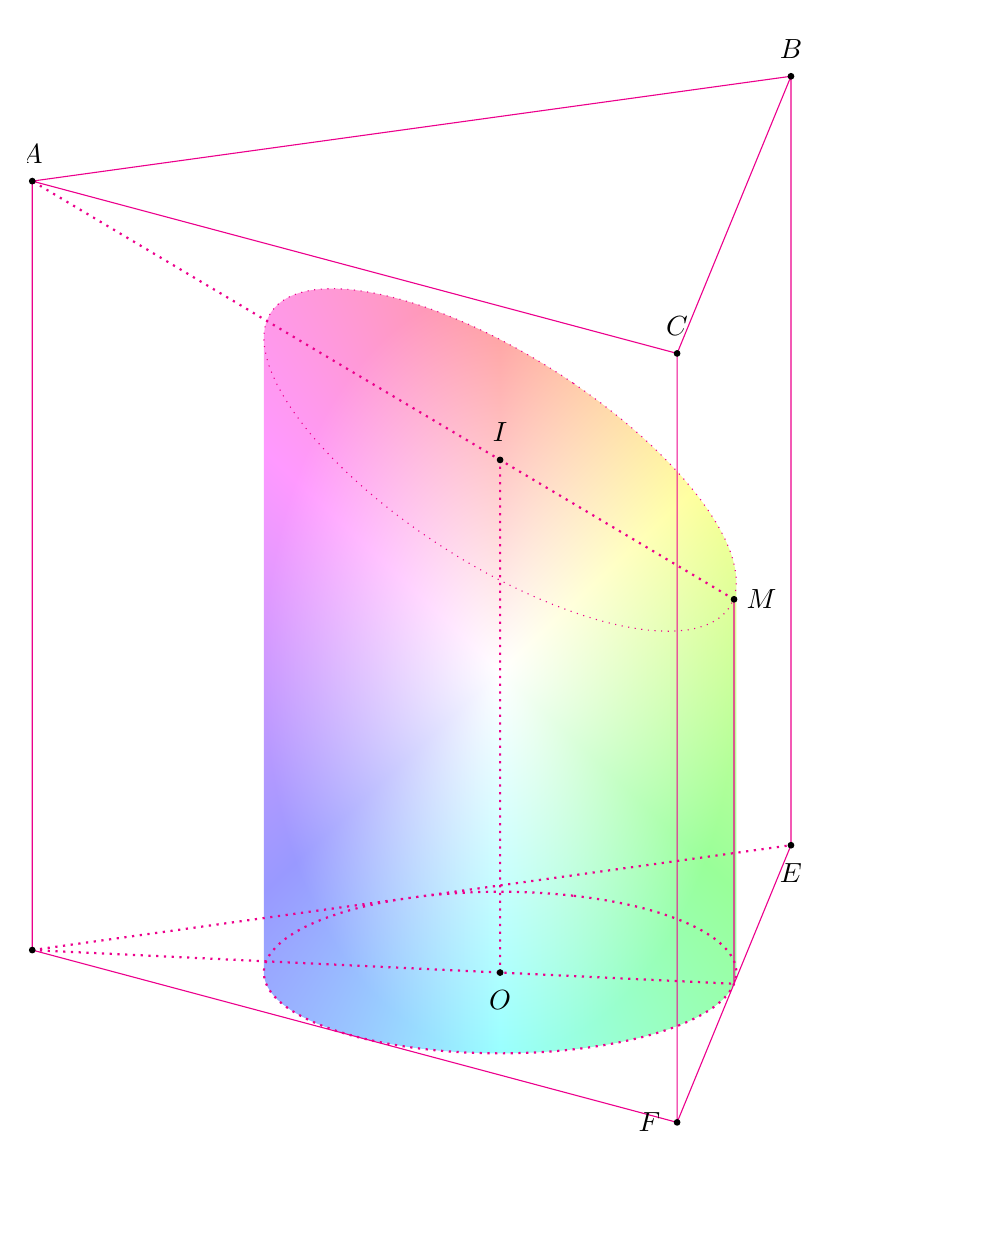
\begin{tikzpicture}
		\def\l{-72}
		\clip(-6,-3)rectangle (6,12);
		\tdplotsetmaincoords{70}{\l}
		\begin{scope}[tdplot_main_coords,>=stealth,magenta]
			\def\r{6}
			\foreach \m/\g in {E/100,D/220,F/340}{
				\path({\r*cos(\g)},{\r*sin(\g)},0)coordinate(\m);
			}
			\path($(D)!0.5!(F)$)coordinate(m)(0,0,{\r*sqrt(3)/2})coordinate(v)($(F)+2*(v)$)coordinate(C)($(E)+2*(v)$)coordinate(B)($(D)+2*(v)$)coordinate(A)($(m)+(v)$)coordinate(M);
			\foreach \x [count=\j]in{\l,180+\l}{
				\path ({(\r/2)*cos(\x)},{(\r/2)*sin(\x)},0)coordinate(n\j)
				({(\r/2)*cos(\x)},{(\r/2)*sin(\x)},{(\r/2)*(1/sqrt(3))*sin(\x)+2*\r/sqrt(3})coordinate(p\j);
			}
			\path(0,0,0)coordinate(O)(0,0,{2*\r/sqrt(3)})coordinate(I);
			\shade[shading=color wheel white center,opacity=0.6,domain=\l:{180+\l},samples=100,opacity=0.4]plot({(\r/2)*cos(\x)},{(\r/2)*sin(\x)},{(\r/2)*(1/sqrt(3))*sin(\x)+2*\r/sqrt(3})--(n2)--plot[ball color=gray,opacity=0.2,domain=180+\l:360+\l,samples=100]({(\r/2)*cos(\x)},{(\r/2)*sin(\x)},0)--cycle;
			\draw[dotted,thick](E)--(F) (O)--(I)(M)--(B)(0,0,0)circle({\r/2})(E)--(m);
			\draw(F)--(D)--(E) (F)--(C)(B)--(E)(A)--(D)(m)--(M)(A)--(B)--(C)--cycle ;
			\draw[dotted,domain=0:360,samples=100]plot({(\r/2)*cos(\x)},{(\r/2)*sin(\x)},{(\r/2)*(1/sqrt(3))*sin(\x)+2*\r/sqrt(3});
		\end{scope}
		\foreach \d/\g/\v in{M/0/M,A/90/C,B/90/A,C/90/B,D/180/F,E/180/D,F/-90/E,I/90/I,O/-90/O}
		\draw[fill=black](\d)circle(1pt)node[shift={(\g:0.35)}]{$\v$};
	\end{tikzpicture}
\end{document}